\begin{frame}
\frametitle{Problem Complexity}
\begin{itemize}
%\item<1-> We must delve into the notion of hardness which come from the general pure exploration bandit literature.
\item<1-> We define $\Delta_i= |r_i - \tau |$ as in Locatelli et al. (2016).
\item<2-> We define $H_{1} = \sum_{i=1}^{K}\dfrac{1}{\Delta_{i}^{2}}$ and $
H_{2} =\min_{i\in \mathcal{A}}\dfrac{i}{{\Delta_{(i)}^{2}}} $ where $\Delta_{(i)}$ is an increasing ordering of ${\Delta}_{i}$.
%\end{align*}$
%where $(\Delta_{(i)}: i\in\mathcal{A})$ is obtained by arranging $(\Delta_i:i\in\mathcal{A})$ in an increasing order. Also, from \cite{chen2014combinatorial} we have
%\begin{align*}
%H_{CSAR,2}=\max_{i\in\mathcal{A}}\frac{i}{\Delta_{(i)}^2}.
%\end{align*}
%$H_{CSAR,2}$ is the complexity term appearing in the bound for the CSAR algorithm. The relation between the above complexity terms are as follows (see \cite{locatelli2016optimal}):
%
%$H_1$ and $H_2$ is same as the problem complexity defined in \cite{locatelli2016optimal} for the thresholding bandit problem while $H_{CSAR,2}=\max_{i}\frac{i}{\Delta_{(i)}^2}$ is defined in \cite{chen2014combinatorial}. Also we know from \cite{locatelli2016optimal} that,
\item<3-> From {Audibert and Bubeck (2010)} the relationship between $H_1$ and $H_2$ can be derived as,
\begin{align*}
H_{2} \leq H_{1}\leq \log(2K)H_{2} 
%\mbox{ and }
 %H_1 \leq \log(K)H_{CSAR,2}.
\end{align*}
\end{itemize}
\end{frame}

\begin{frame}
\begin{itemize}
\item We define $\Delta_i= |r_i - \tau |$ as in Locatelli et al. (2016).
\item We define $H_{1} = \sum_{i=1}^{K}\dfrac{1}{\Delta_{i}^{2}}$ and $
H_{2} =\min_{i\in \mathcal{A}}\dfrac{i}{{\Delta_{(i)}^{2}}}$ as in Audibert and Bubeck (2010).
\item $H_{\sigma,1}=\sum_{i=1}^{K}\frac{\sigma_{i}+\sqrt{\sigma_{i}^{2}+(16/3)\Delta_{i}}}{\Delta_{i}^{2}}$.
\item $H_{\sigma,2}=\max_{i\in \mathcal{A}} \frac{i}{\tilde{\Delta}_{(i)}^{2}}$ where $\tilde{\Delta}_{i}^{2}=\frac{\Delta_{i}^{2}}{\sigma_{i}+\sqrt{\sigma_{i}^{2}+(16/3)\Delta_{i}}}$.
\item From Audibert and Bubeck (2010) we can show $H_{2} \leq H_{1}\leq \log(2K)H_{2}$ and $H_{\sigma,2}\le H_{\sigma,1} \le \log(2K) H_{\sigma,2}$.
\end{itemize}
\end{frame}

\begin{frame}
\frametitle{Problem Complexity}
\begin{itemize}
\item<1-> For a variance aware algorithm we define $H_{\sigma , 1}$ ( as in {Gabillon et al. (2011)}) that incorporates reward variances into its expression as:
\begin{align*}
 H_{\sigma,1}=\sum_{i=1}^{K}\frac{\sigma_{i}+\sqrt{\sigma_{i}^{2}+(16/3)\Delta_{i}}}{\Delta_{i}^{2}}.
\end{align*}

\item<2-> Finally, analogous to $H_{2}$, we introduce $H_{\sigma,2}$, such that $
H_{\sigma,2}=\max_{i\in \mathcal{A}} \frac{i}{\tilde{\Delta}_{(i)}^{2}}$ , where $\tilde{\Delta}_{i}^{2}=\frac{\Delta_{i}^{2}}{\sigma_{i}+\sqrt{\sigma_{i}^{2}+(16/3)\Delta_{i}}}$,  $(\tilde{\Delta}_{(i)})$ is an increasing ordering of $(\tilde{\Delta}_{i})$.

\item<3-> From {Audibert and Bubeck (2010)}, we can show that
\begin{align*}
H_{\sigma,2}\le H_{\sigma,1} \le \log(2K) H_{\sigma,2}.
\end{align*}


\item<4-> Note that $H_1 , H_2 $ and $H_{\sigma,1}, H_{\sigma,2}$ are not directly comparable to each other except in a special case when variances and gaps $(\Delta_i)$ are very low we can say that $H_{\sigma,1} < H_{1} $.

\end{itemize}
\end{frame}



\begin{frame}
\frametitle{Expected Loss of AugUCB}

\begin{theorem}
For $K\geq 4$ and $\rho={1}/{3}$,
the expected loss of the AugUCB algorithm is given by,
\begin{align*}
\E[\Ls(T)]
& \leq 2KT \exp\bigg(- \frac{T}{4096 \log( K\log K) H_{\sigma,2}} \bigg).
\end{align*}
\end{theorem}


\begin{table}[b]
\caption{AugUCB vs.\ State of the art}
\label{tab:regret-bds}
\begin{center}
\begin{tabular}{|p{1.5cm}|p{6.4cm}|p{1.5cm}|}
% \toprule
\hline
Algorithm  & Upper Bound on Expected Loss & Oracle \\
% \midrule
\hline
%\hline
AugUCB      &$ \exp\left(- \frac{T}{4096 \log(K\log K)H_{\sigma,2}} + \log\left(2KT\right) \right) $ & No\\
%\hline
\hline
UCBEV		&$\exp\left(-\frac{1}{512}\frac{T-2K}{H_{\sigma,1}} + \log\left(6KT\right)\right)$ & Yes\\
%\midrule
%\hline
\hline
APT         &$\exp\left(-\frac{T}{64 H_1}+2\log((\log(T)+1)K)\right)$ & No\\
% \midrule
%\hline
\hline
UCBE		&$\exp\left(-\frac{T-K}{18 H_1} - 2\log(\log(T)K\right)$ &  Yes\\
%\midrule
\hline

%\bottomrule
\end{tabular}
\end{center}
\end{table}
\end{frame}

%\begin{frame}
%\frametitle{Concentration Bounds}
%\begin{itemize}
%\item<1-> Let $X_{1}, . . . , X_{n}$ be random variables with common support $[0, 1]$ and such that $E[X_{t} |X_{1}, . . . , X_{t-1}] = r_i$. Let $\hat{r}_i = \dfrac{X_{1} +,....,+ X_{n}}{n}$. Then for all $c \geq 0$,
%\begin{align*}
%\mathbb{P} \lbrace \hat{r}_i \geq r_i + c \rbrace \leq \exp{(-2c^{2}n)}\\
%\mathbb{P}\lbrace \hat{r}_i \leq r_i - c \rbrace \leq \exp{(-2c^{2}n)}
%\end{align*}
%
%\item<2-> Along with the above information if we know that $\text{Var}[X_{t} |X_{1}, . . . , X_{t-1}]=\sigma_i^2$ then Bernstein inequality gives us,
%\begin{align*}
%\mathbb{P} \lbrace \hat{r}_i \geq r_i + c \rbrace \leq \exp{(-\dfrac{c^{2}n}{2\sigma_i^2 +\frac{2c}{3}})}\\
%\mathbb{P}\lbrace \hat{r}_i \leq r_i - c \rbrace \leq \exp{(-\dfrac{c^{2}n}{2\sigma_i^2 +\frac{2c}{3}})}
%\end{align*}
%
%\end{itemize}
%\end{frame}

\begin{frame}
\frametitle{Sketch of the proof}
\begin{figure}
%\caption{AugUCB arm elimination}
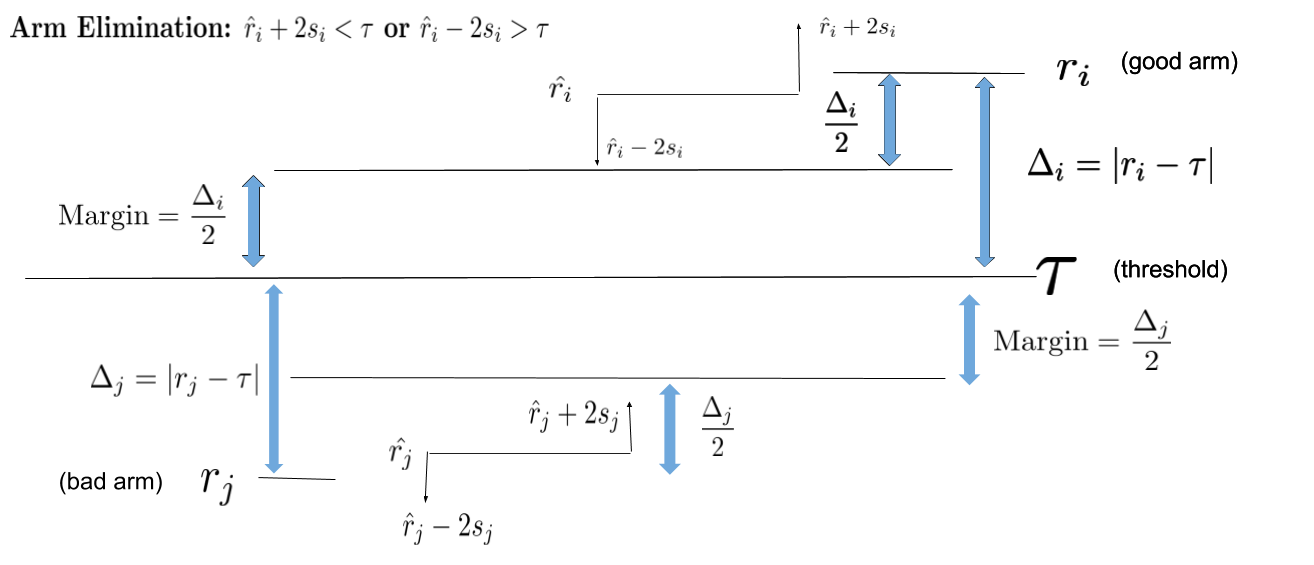
\includegraphics[scale=0.278]{img/ArmElim3.png}
\end{figure}
%\begin{itemize}
%\item<1-> The proof comprises of two modules. In the first module we investigate the necessary conditions for arm elimination within a specified number of rounds, which is motivated by the technique in UCB-Imp. 
% 
%\item<2-> We bound the arm-elimination probability by Bernstein inequality (as in {Audibert et al. (2009)}) rather that the Chernoff-Hoeffding bounds (used in UCB-Imp). 
%
%\item<3-> In the second module,we define a favourable event that will yield an upper bound on the expected loss and use union bound and module-1 (on the arm elimination probability) to derive the result through a series of simplifications.
%\end{itemize}
\end{frame}



